% Panel captions for the graph-incompleteness validation figures.
% Every number quoted here is read from validation-incompleteness/results/*.json
% by make_figures.py; nothing is drawn by hand and no curve is fitted.

\begin{figure*}[!htbp]
    \centering
    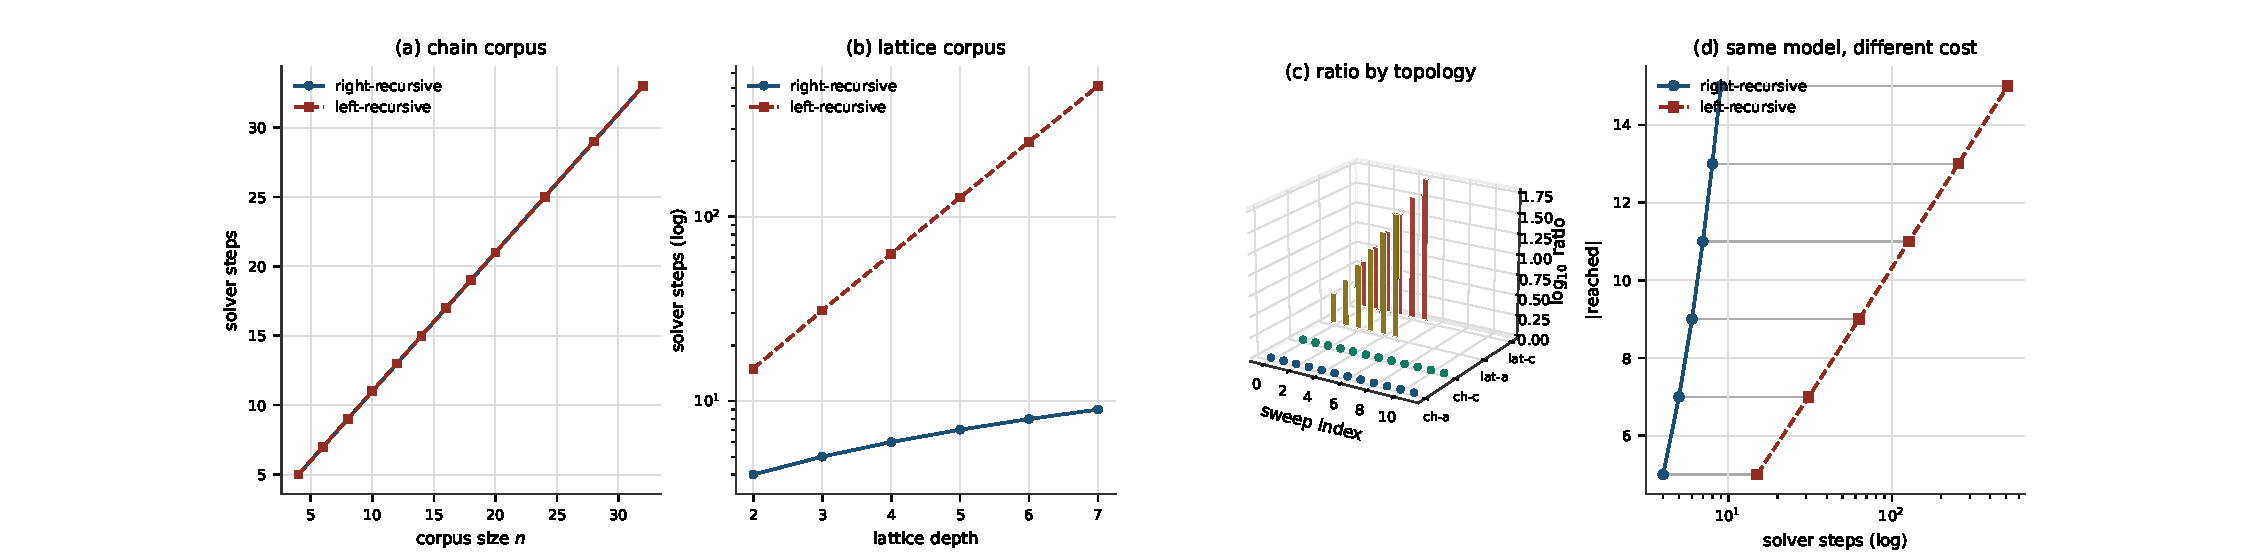
\includegraphics[width=\textwidth]{figures/panel_1_recursion_shape.pdf}
    \caption{\textbf{Recursion shape is free on path-shaped corpora and expensive on branching ones, at an identical least model.}
    Both shapes compute reachability under the same transitive rule on the same corpora; the sweep varies only the direction of the recursion, so every difference plotted is a difference in cost and not in what was computed.
    (\textbf{A})~Solver steps against corpus size on the chain, $n = 4$ to $32$. The two curves coincide exactly at every point: the right-recursive traversal costs $4 \to 32$ steps and the left-recursive traversal costs $4 \to 32$ steps, a ratio of exactly $1.000$ at all twelve sizes and under both the acyclic and cyclic variants. A chain gives each node exactly one successor, so the left-recursive agenda never re-derives and the cost half of \Cref{prop:recursion-shape} is structurally invisible.
    (\textbf{B})~The same two shapes on a diamond lattice of depth $2$ to $7$, logarithmic ordinate. The right-recursive traversal costs $4 \to 9$ steps while the left-recursive traversal costs $15 \to 511$, and the separation grows monotonically with depth. The claim is the same claim; only the corpus topology changed.
    (\textbf{C})~The cost ratio $\text{left}/\text{right}$ across all four topologies, $\log_{10}$ ordinate. The two chain series are drawn as flat marker rows at $\log_{10} 1 = 0$ rather than as bars of zero height, so that \emph{measured and equal to one} remains visually distinct from \emph{not measured}. The lattice ratios climb to $31.9$ (acyclic) and $56.8$ (cyclic).
    (\textbf{D})~Answer-set size against solver steps on the cyclic lattice, logarithmic abscissa, with grey connectors joining the two shapes at each depth. The connectors are horizontal at every depth: the two traversals reach identical least models ($|{\text{reached}}| = 5 \to 15$) at costs differing by up to a factor of $57$. Without this chart (\textbf{A})--(\textbf{C}) would not be a cost comparison but a comparison of two different computations.
    The practical reading is that a benchmark assembled from chain-shaped corpora cannot distinguish the two recursion shapes at all.}
    \label{fig:panel-recursion-shape}
\end{figure*}

\begin{figure*}[!htbp]
    \centering
    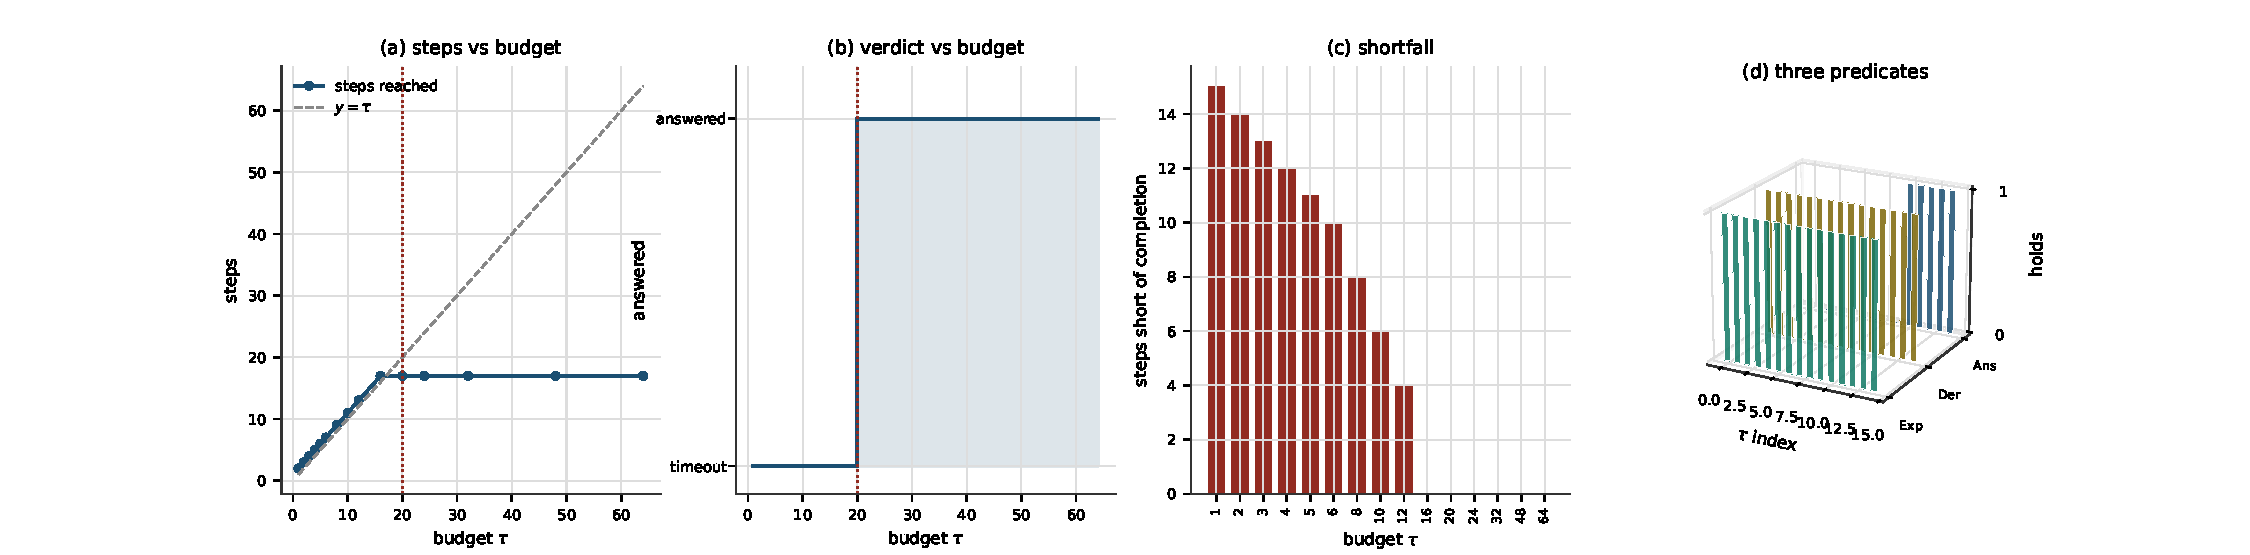
\includegraphics[width=\textwidth]{figures/panel_2_budget.pdf}
    \caption{\textbf{The budget is the only one of the three predicates that carries a clock.}
    A single question is evaluated against a single model and a single corpus of $16$ assertions at fifteen budgets $\tau \in \{1,\dots,64\}$. Nothing but $\tau$ varies across the sweep, so every change in verdict is attributable to the budget alone.
    (\textbf{A})~Steps reached against $\tau$, with the diagonal $y = \tau$ for reference. Below threshold the traversal halts one step past its budget and tracks the diagonal; from $\tau = 20$ onward it saturates at $17$ steps and the curve leaves the diagonal, because the computation has finished rather than been cut off.
    (\textbf{B})~The verdict as a function of $\tau$. Exactly two labels are ever observed --- \textsc{answered} and \textsc{timeout} --- and the transition is a single monotone step at $\tau = 20$ (dotted line). The verdict changes with the budget alone, holding language, semantics, model and corpus fixed.
    (\textbf{C})~Steps short of completion at each budget, coloured by outcome. The shortfall falls from $15$ at $\tau = 1$ to $0$ at threshold and stays there, and the bar colour switches at the same point; the two encodings of the same transition are drawn together as a consistency check on (\textbf{B}).
    (\textbf{D})~$\mathrm{Exp}$, $\mathrm{Der}$ and $\mathrm{Ans}_\tau$ over the same fifteen budgets. The first two are flat at $1$ across the entire sweep --- the question remains expressible and remains derivable no matter how little time is allowed --- while only $\mathrm{Ans}_\tau$ moves. This is the operational content of \Cref{thm:independence}: a system that reports one number cannot say which of the three it means, and only the third has any dependence on the clock.}
    \label{fig:panel-budget}
\end{figure*}

\begin{figure*}[!htbp]
    \centering
    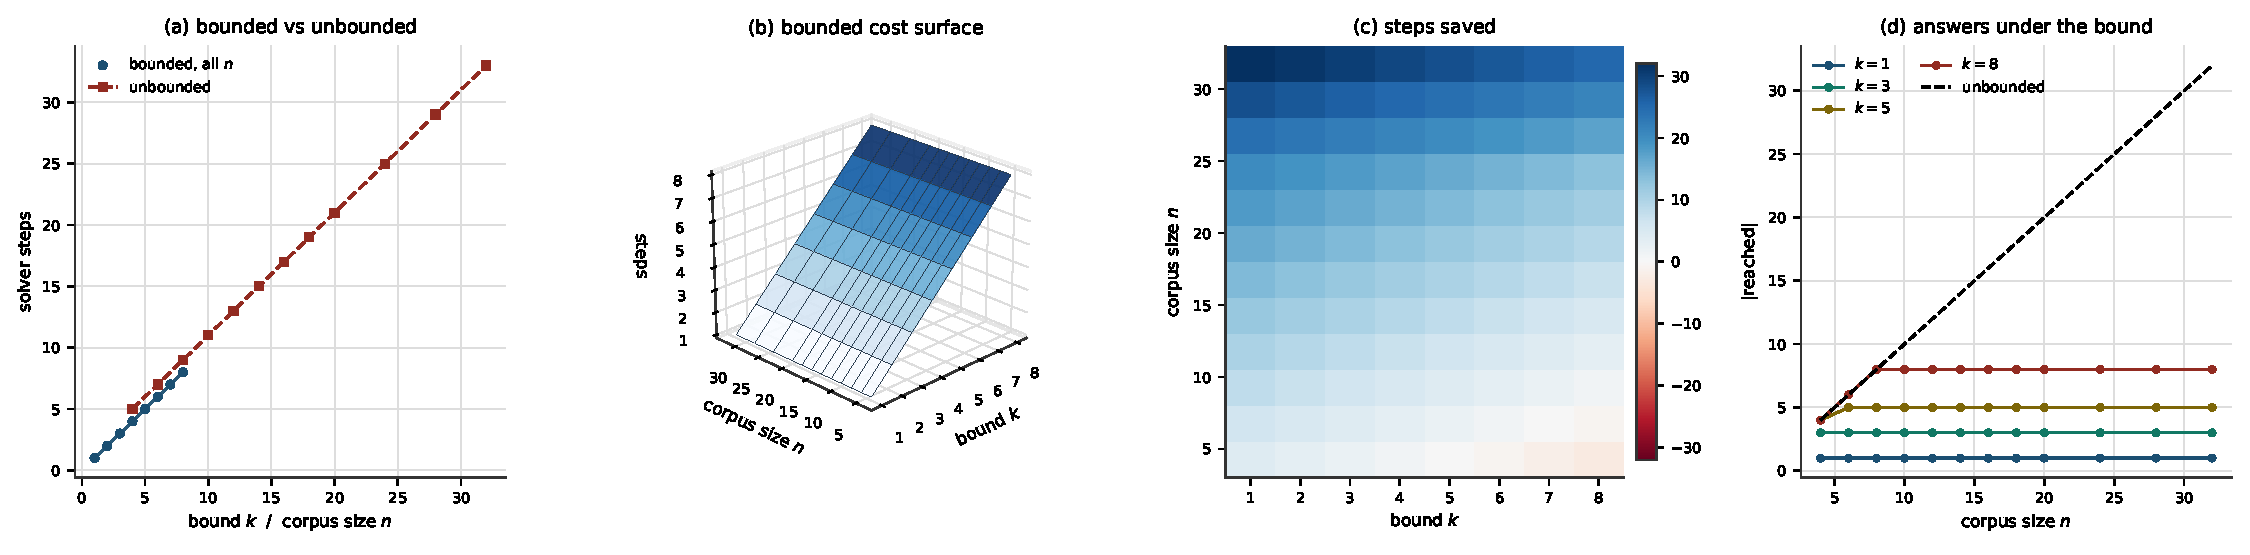
\includegraphics[width=\textwidth]{figures/panel_3_bounded.pdf}
    \caption{\textbf{A bounded query costs the bound and not the corpus, which inverts the usual expectation on $90$ of $96$ measured cells.}
    The grid crosses eight bounds $k \in \{1,\dots,8\}$ with twelve corpus sizes $n \in \{4,\dots,32\}$; the unbounded reachability query is run on the same twelve corpora for comparison.
    (\textbf{A})~Bounded cost against $k$ overlaid on unbounded cost against $n$. The bounded series is exactly $k$ steps at every one of the $96$ cells, independent of $n$; the unbounded series grows as $n+1$, from $5$ to $33$ steps.
    (\textbf{B})~The bounded cost surface over $(k, n)$. It is a ramp in $k$ and exactly flat in $n$: a plane, not a curved surface. The flatness in $n$ is the content of \Cref{prop:bounded-cheaper}, and it is a property of the query, not of the corpus it runs against.
    (\textbf{C})~Steps saved, $\text{unbounded} - \text{bounded}$, on a diverging scale centred at zero. The blue region is the inversion of \Cref{cor:inversion}: the syntactically more restrictive query is the cheaper one, over $90$ of $96$ cells. The six red cells are the small-$n$, large-$k$ corner where the bound exceeds the corpus and buys nothing; drawing them rather than cropping them is what makes the blue region a finding rather than a definition.
    (\textbf{D})~Answers returned under each bound, against unbounded reachability. Each bounded series saturates at exactly $k$ reachable nodes while the unbounded series grows without limit, which is the price of the inversion in (\textbf{C}) and the reason it is a trade rather than a free improvement.}
    \label{fig:panel-bounded}
\end{figure*}

\begin{figure*}[!htbp]
    \centering
    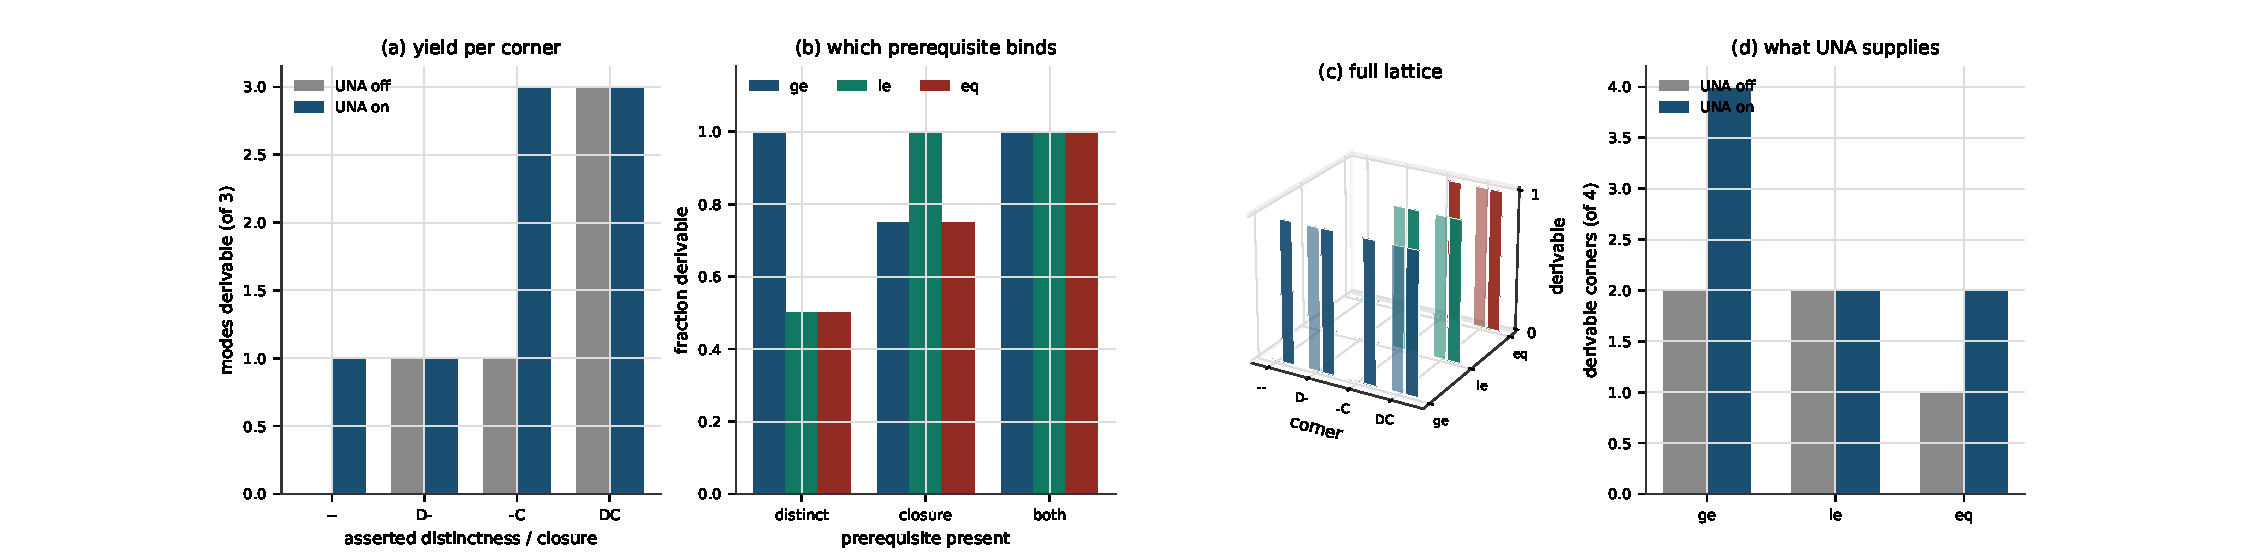
\includegraphics[width=\textwidth]{figures/panel_4_counting.pdf}
    \caption{\textbf{The three counting modes have different semantic prerequisites, and the unique-name assumption silently supplies one of them.}
    All $24$ cells cross three modes ($\mathrm{ge}$, $\mathrm{le}$, $\mathrm{eq}$) with the four corners of asserted distinctness and closure and with the unique-name assumption off and on. Corner labels read \texttt{--}, \texttt{D-}, \texttt{-C}, \texttt{DC} for neither, distinctness only, closure only, and both.
    (\textbf{A})~Modes derivable at each corner, under each UNA regime. With UNA off the yield rises $0 \to 1 \to 1 \to 3$ across the corners; with UNA on the empty corner already yields $1$ and the closure-only corner yields all $3$. The lift is the assumption doing semantic work that the corner did not assert.
    (\textbf{B})~The fraction of cells each mode clears once a given prerequisite is present. The pattern is the signature of \Cref{prop:counting-split}: $\mathrm{ge}$ reaches $1.00$ given distinctness alone, $\mathrm{le}$ reaches $1.00$ given closure alone, and $\mathrm{eq}$ reaches $1.00$ only when both are present, sitting at $0.50$ and $0.75$ respectively when given one.
    (\textbf{C})~The full $24$-cell lattice over mode, corner and UNA regime, with the UNA-off cells drawn translucent behind the UNA-on cells. The satisfying corners are $\{\texttt{D-}, \texttt{DC}\}$ for $\mathrm{ge}$, $\{\texttt{-C}, \texttt{DC}\}$ for $\mathrm{le}$, and $\{\texttt{DC}\}$ alone for $\mathrm{eq}$; $13$ of $24$ cells are derivable.
    (\textbf{D})~Derivable corners per mode with UNA off against UNA on. Turning the assumption on lifts $\mathrm{ge}$ from $2$ to $4$ corners and $\mathrm{eq}$ from $1$ to $2$, and leaves $\mathrm{le}$ unchanged at $2$ --- exactly the modes whose prerequisite is distinctness, and exactly the mode whose prerequisite is not. The cells are keyed on \emph{asserted} rather than effective distinctness precisely so that this substitution is visible; keying on the effective value would have hidden it, which is the inheritance \Cref{prop:inherited-una} names and \Cref{rem:una-scope} bounds.}
    \label{fig:panel-counting}
\end{figure*}

\begin{figure*}[!htbp]
    \centering
    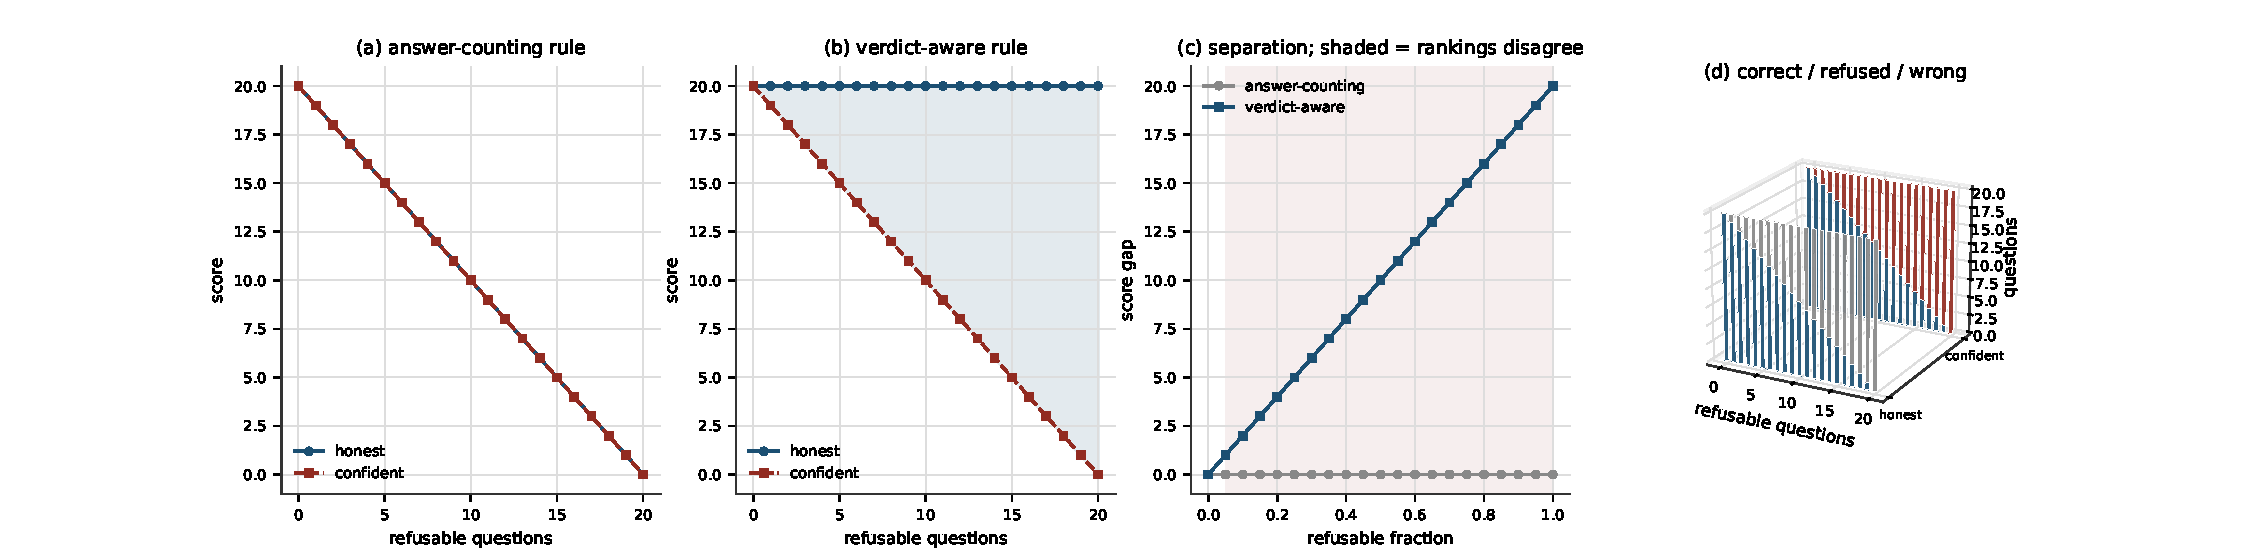
\includegraphics[width=\textwidth]{figures/panel_5_scoring.pdf}
    \caption{\textbf{An answer-counting benchmark cannot distinguish an honest refuser from a confidently wrong system, and the ordering it induces is reversed by a verdict-aware rule.}
    Twenty questions are scored at twenty-one compositions, from all answerable to all refusable. The two systems differ in exactly one respect: on a question it cannot support, the honest system refuses and the confident system returns a certified empty answer set.
    (\textbf{A})~Both systems under the answer-counting rule. The two curves coincide exactly at all twenty-one mixes, falling together from $20.0$ to $0.0$; the gap is $0.00$ everywhere. The rule cannot see the difference between the two systems because the difference is in the verdict and the rule reads only the answer.
    (\textbf{B})~The same two systems on the same data under a verdict-aware rule. The honest system holds at $20.0$ across every mix while the confident system falls to $0.0$, the shaded region being the deficit the first rule discarded.
    (\textbf{C})~The gap under each rule against the refusable fraction. The answer-counting gap is flat at $0.00$; the verdict-aware gap rises linearly to $20.0$, exactly proportional to the number of refusable questions. The shaded band marks the mixes at which the two rules \emph{rank the two systems differently} --- all twenty mixes with at least one refusable question. The ordering reversal, not the size of the gap, is the claim of \Cref{prop:compare-refusals}.
    (\textbf{D})~The mechanism behind (\textbf{C}): each system's twenty questions decomposed into answered-correctly, refused, and answered-wrongly. Both systems attempt the same total at every mix, and the two stacks are identical in height and differ only in what the second component \emph{is}. The confident system's second stack is wrong answers where the honest system's is refusals, and it is precisely this component that the answer-counting rule credits and the verdict-aware rule debits.}
    \label{fig:panel-scoring}
\end{figure*}

\begin{figure*}[!htbp]
    \centering
    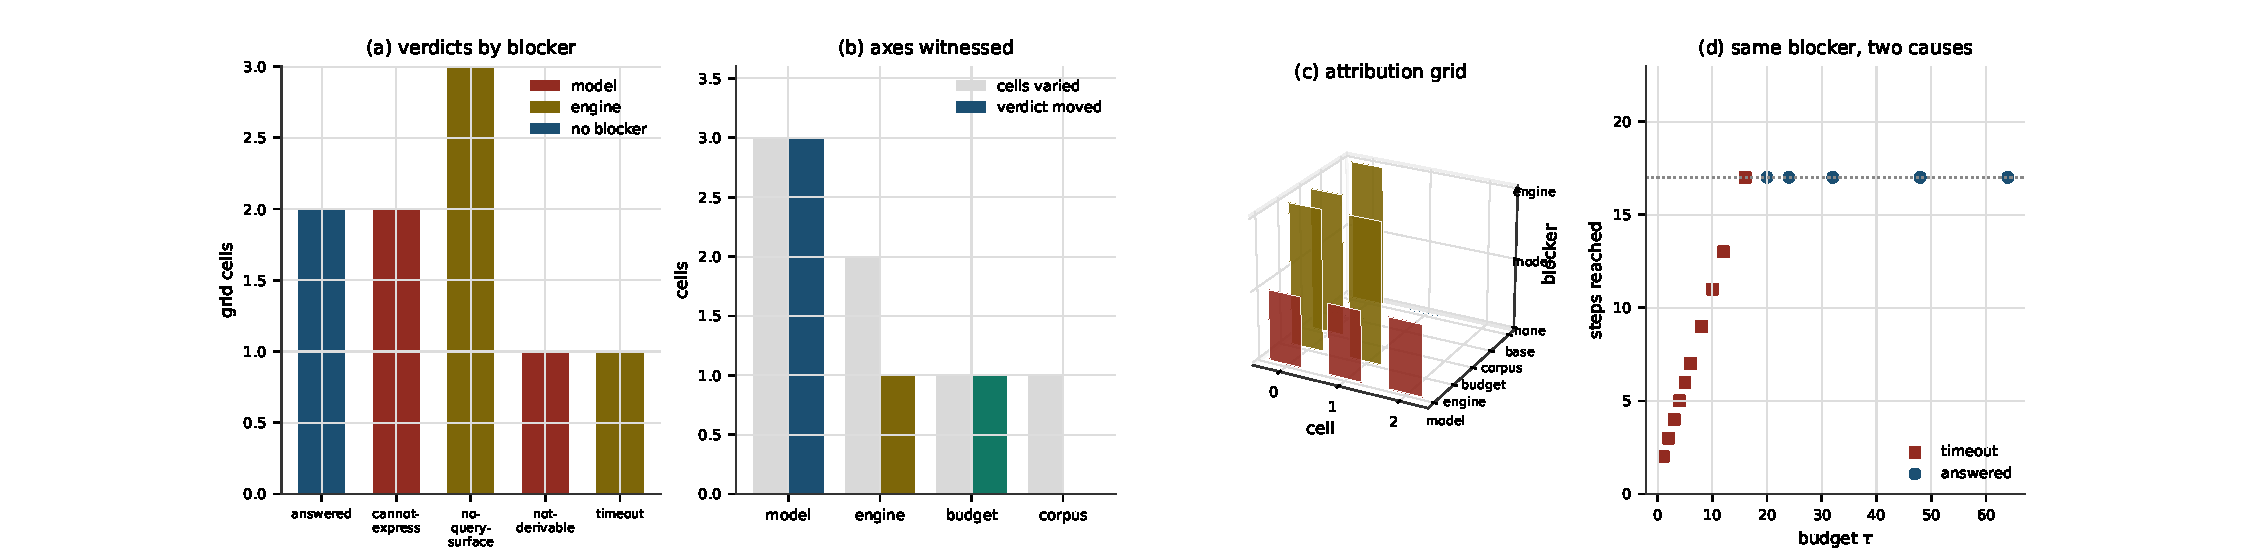
\includegraphics[width=\textwidth]{figures/panel_6_blockers.pdf}
    \caption{\textbf{Varying one axis at a time attributes a refusal to model, engine or budget --- and shows that two of the trichotomy's cases are not separated by the blocker alone.}
    Nine settings are evaluated, each differing from a stated baseline in exactly one of model, engine, corpus or budget, and each contrast is recorded as a pair so that a verdict is compared against the verdict it replaced rather than merely inspected.
    (\textbf{A})~Verdicts observed across the grid, stacked by the blocker assigned to each. Five labels occur, and the two \textsc{answered} cells alone carry no blocker: no case with an answer is attributed to an obstruction, which is the non-degeneracy of \Cref{thm:nondegeneracy} holding across the grid.
    (\textbf{B})~Cells varied against cells whose verdict actually moved, per axis. Model moves $3$ of $3$, budget $1$ of $1$, engine $1$ of $2$, and corpus $0$ of $1$. The bars are drawn side by side rather than overlaid because an axis that moves every cell would otherwise hide its own baseline. Two negative results are recorded here rather than removed: swapping the engine under a counting question changes nothing, since neither engine lowers \textsc{counting} and the question is refused before either is consulted; and emptying the extension of a declared concept yields \textsc{answered} with an empty answer set rather than any blocker at all.
    (\textbf{C})~The attribution grid, cell by cell, coded by blocker. Only two of the three values in \Cref{def:blocker} are ever produced: \emph{blocked-by-model} and \emph{blocked-by-engine}. \emph{Blocked-by-corpus} is not reachable through the evaluation order of \Cref{def:evaluation} at all --- no clause emits a label that maps to it --- so the trichotomy is exhaustive over blockers but not over what the evaluator can actually report.
    (\textbf{D})~The budget sweep replotted against outcome. A timeout and a missing lowering are both attributed to \emph{blocked-by-engine}, so the blocker alone does not distinguish \emph{cannot compile this question} from \emph{was not given time to finish it}; the two are separated only by the verdict label that accompanies it. A repair recommendation read off the blocker without the label would therefore be ambiguous between writing a compiler and raising a number.}
    \label{fig:panel-blockers}
\end{figure*}
